\section{Activation-Function Inductive Bias}
\label{sec:verification}

\subsection{Motivation: Polynomial Kolmogorov-Arnold Networks}

Ahmed \& Davis \cite{ahmed2026polynomial} study why small neural networks
struggle to \emph{learn} the GoL transition rule despite minimal networks
being known to \emph{represent} it exactly with only a handful of
hand-set parameters \cite{springer2021minimal}. They argue that the GoL
update is a non-monotonic function of live-neighbor count $N$ --- flat at
zero for $N \in \{0,1\}$, rising sharply for $N \in \{2,3\}$, and flat at
zero again for $N \geq 4$ --- which a monotonic activation such as ReLU can
only approximate piecewise, requiring many units and a fortunate
initialization (a ``winning ticket'') to succeed reliably. They show that
replacing ReLU with a \emph{learnable second-degree polynomial} activation,
\[
  \phi(x) = w_0 + w_1 x + w_2 x^2,
\]
lets a minimal CNN --- one $3\times3$ circularly-padded convolution, one
$1\times1$ convolution, and a final $1\times1$ convolution with sigmoid
output --- learn GoL reliably on a $32\times32$ toroidal grid, whereas the
same architecture with ReLU activation fails almost completely.

\subsection{Independent reproduction}
\label{sec:reproduction}

Before attempting to transfer this idea into our larger CNN-Transformer, we
independently verify the paper's central claim on our own $40\times40$
toroidal setup, using a from-scratch reimplementation (available in
\texttt{poly\_activation\_verify/}, kept deliberately separate from the main
codebase) with no dependency on our own GoL simulator or model code. We
build the minimal $L(1,m{=}1)$ architecture described above and train two
variants --- identical in every respect except the activation function used
at the two hidden activation sites --- with plain single-step teacher
forcing (binary cross-entropy, Adam, learning rate $10^{-3}$, batch size
$8$) on a small dataset of 100 training / 20 validation random grids
(density sampled uniformly in $[0.1, 0.9]$), across 10 random seeds per
activation.

\begin{table}[htbp]
\centering
\begin{tabular}{lrrrr}
\toprule
Activation & Parameters & Success rate & Mean epochs to converge & Mean final accuracy \\
\midrule
ReLU       & 25 & 1/10  & 159.0 (of successful run) & 89.39\% \\
Polynomial & 34 & 10/10 & 185.6 & 100.00\% \\
\bottomrule
\end{tabular}
\caption{Reproduction of Ahmed \& Davis \cite{ahmed2026polynomial} on our
own $40\times40$ toroidal grid and independent implementation. Parameter
counts (25 and 34) match the paper's reported minimal-network sizes
exactly. ``Success'' is defined as reaching $\geq 99.99\%$ validation cell
accuracy for two consecutive epochs, within 500 epochs.}
\label{tab:relu-vs-poly}
\end{table}

\begin{figure}[htbp]
  \centering
  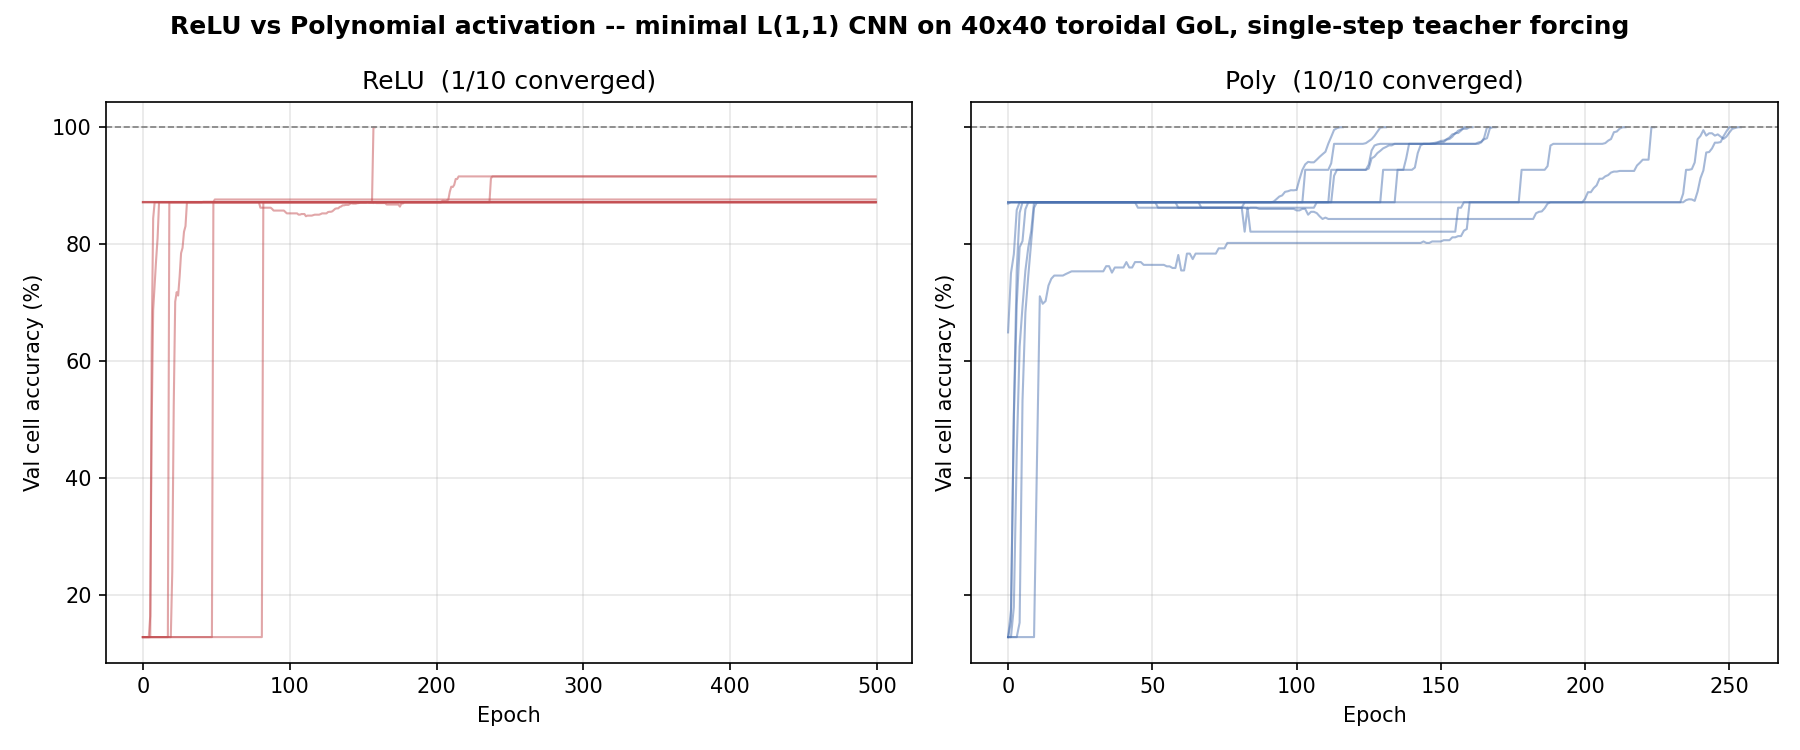
\includegraphics[width=0.9\textwidth]{figures/relu_vs_poly_convergence.png}
  \caption{Validation accuracy over training, all 10 seeds. ReLU (left)
  plateaus around 87--92\% for 9 of 10 seeds and never escapes; polynomial
  activation (right) reaches 100\% accuracy on every seed.}
  \label{fig:relu-vs-poly}
\end{figure}

The reproduction (Table~\ref{tab:relu-vs-poly}, Figure~\ref{fig:relu-vs-poly})
confirms the paper's claim under an independent implementation, a different
grid size, and a different (and much smaller) training set than the
original paper used: ReLU converges to perfect accuracy on only 1 of 10
seeds, plateauing at 87--92\% cell accuracy on the rest, while the
polynomial activation converges to perfect accuracy on all 10 seeds,
typically within 120--260 epochs (each run completing in 1--2 seconds on
CPU, given the network's tiny size).

\subsection{Negative result: transferring the polynomial activation to the multi-step model}
\label{sec:v11}

Given the clean reproduction in Section~\ref{sec:reproduction}, we attempted
to transfer the polynomial activation into the CNN feature-extraction stage
of the full CNN-Transformer architecture (Section~\ref{sec:architecture}),
at V8's parameter budget ($d_{\text{model}}=64$, 4 layers): replacing the
two GELU activations in Stage 1 with the same learnable
$\phi(x)=w_0+w_1x+w_2x^2$ used in Section~\ref{sec:reproduction}, while
leaving the Transformer encoder's GELU unchanged. This adds only $288$
parameters over the baseline V8 architecture ($292{,}176$ vs.\ $291{,}888$),
so any accuracy change can be attributed to the activation rather than to
capacity. The model was trained from scratch with the same scheduled
sampling recipe used for V10 (Section~\ref{sec:training-evolution}): $K=3$
unrolled steps, $p: 0 \to 1$ over training, learning rate $10^{-4}$.

Training was \emph{not} stable. By epoch 5, validation metrics were
promising (F1 $=0.89$, born-accuracy $86.8\%$, validation loss $0.227$) ---
already close to V8's converged performance after only 5 epochs from
scratch. However, by epoch 10 the model had regressed sharply (validation
loss $0.491$, F1 $0.39$), and by epoch 15 it had diverged further
(validation loss $1.045$, F1 $0.17$), while per-epoch wall-clock time grew
roughly five-fold over the same interval. Training loss remained flat
throughout ($\approx 0.21$) even as validation loss exploded, indicating
the divergence is specific to the clean single-step evaluation distribution
rather than a general optimization failure.

We hypothesize this reflects an interaction between the polynomial
activation and the multi-step scheduled-sampling training loop that is
absent from the single-step setup verified in
Section~\ref{sec:reproduction}: the $w_2 x^2$ term is unbounded and,
unlike a saturating activation such as GELU, has no mechanism to suppress
large intermediate activations. Once scheduled sampling begins feeding the
model's own (initially imperfect) predictions back as input to later
unrolled steps, any activation values that drift into a regime where the
quadratic term dominates are amplified rather than clipped, compounding
across the $K=3$ steps in a manner structurally similar to the STE failure
mode identified for V6 (Section~\ref{sec:training-evolution}). We did not
observe this instability in Section~\ref{sec:reproduction} because that
experiment uses pure single-step teacher forcing with no autoregressive
feedback loop.

This negative result was not pursued further within the scope of this
report; we record it here as we consider the failure mode informative in
its own right, and as a caution against assuming an inductive-bias fix
verified in a minimal single-step setting will transfer unmodified to a
larger multi-step training regime. Candidate fixes --- left to future work
--- include bounding the quadratic coefficient (e.g.\ a saturating variant
$\phi(x) = w_0 + w_1 x + w_2 x^2/(1+x^2)$), using a separate, smaller
learning rate for the polynomial coefficients, or first verifying
single-step (teacher-forcing-only) training at V8/V10 scale before
introducing scheduled sampling.
